\section{Program and Design}

Content   \cite{Pellis1997}.  

%%%%%%%%%%%%%%%%%%%%%%%%%%%%%%%%%%%%%%%%%%%%%%%%%%%%%%%%%%%%%%%%%%
%%%%%%%%			OBJECTIVES METHODOLOGY AND RESEARCH
%%%%%%%%%%%%%%%%%%%%%%%%%%%%%%%%%%%%%%%%%%%%%%%%%%%%%%%%%%%%%%%%%%

\subsection{Objectives}

\paragraph{}
The objective of this reearch project is to attempt to answer the overall question of whether a low voltage DC power distribution system could be implemented. A secondary objective is to relate this project directly to renewable energy generation. Additionally it needs to be kept costs low and replace expensive construction of designs with realistic simulations. 

\subsection{Methodology}

\paragraph{}
In order to complete this task within a timely manner and ensure all aspects are thoroughly considered and discussed, a clear guideline of tasks musts be followed. Additionally, these tasks will need to specifically address the objectives that the research proposal addresses. As discussed in Section 3, there are five broad questions that are being addressed throughout the two semesters of this thesis. The methodology of the thesis is based around a combination of physical and theoretical testing. A reliance on previous research and design recommendations will be important as low-voltage DC systems is an area that has been researched consistently in recent years with the increase in renewable energy systems and increasingly efficienct. 

\paragraph{}
The five separate questions are related to the same solution. Initial stages of the project require extensive research at the possibilities and theories behind a purely DC system. Once a strong idea of the possibilities and previous papers were analysed a general analysis of whether or not 48V is the ideal voltage level is secondary. To do this, it will be predominately theoretical with voltage loss caclualtions over standard cable lengths. Once this is the decided the next stage can be followed. Photo-voltaic systems are a common consideration when wanting to directly generate DC power. This project will use resources available to assess the options with solar panels and whether each option is suitable for applications. 

\paragraph{}
The next stage and the main application that this project will be assessing. Ideally, a prototype will be constructed and tested that simulates a photo-voltatic array's ability to generate DC electricity. Then a battery system and DC-DC converter need to be designed in order to power an LED circuit. The reason for a solar array simulation is that with the low budget of this project, buying solar arrays is not a solution. These devices needed to be designed, built and tested to learn the extent of cable length and number of electronics able to be powered. The final consideration is what applications the design could be used for; whether that be residential, commercial and industrial. In order to calculate this I can use my personal knowledge of power systems from my work role as well as access to industry power calculation software. 

\paragraph{}
Testing will be done whilst at University with access to specialised equipment whereever possible. This will allow for quick access to the electrical store as well as experienced individuals close by for guidance. If a test is required, similar to how the Unversity structures their practicals, I will write a brief practical document including aim, background, equipment, steps and a method of recording data. Safety is of the utmost priority when performing experiments especially when dealing with power systems. Clear risk assessments will be required before any test can be performed. 

\begin{figure}[H]
\hfill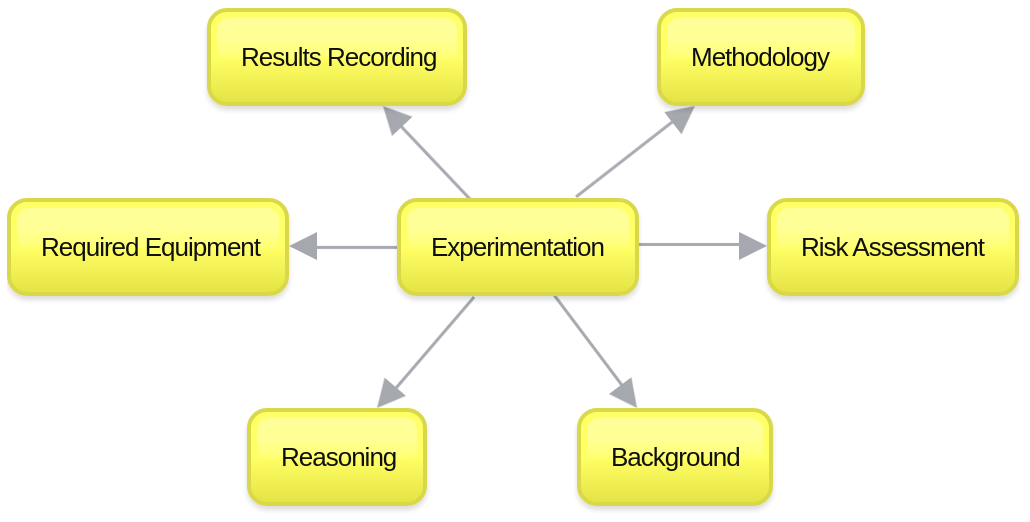
\includegraphics[width = 160mm]{images/Practical_Planning}\hspace*{\fill}
\caption{Considerations for a Practical Procedure}
\label{fig:EmergingTrends}
\end{figure}     

\subsection{Research Plan}

\paragraph{}
A large majority of the project will be through simulations utilising Matlab, PowerCad5, Dialux4.11 and PowerPac. This is due to power systems electronics being relatively expensive and large skale testing out of the financial scope of this project. Ideally, a full system would be built with Photo-Voltaic cells, battery, controller, DC-DC converters and connections to appliances, however finances are unlikely to allow this. Figure 4 below shows the individual areas that will require designs and testing. 

\begin{figure}[H]
\hfill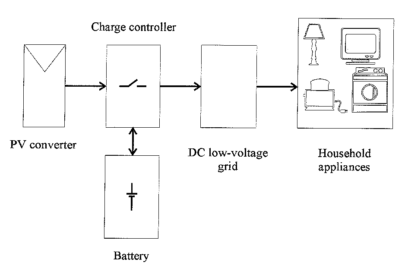
\includegraphics[width = 160mm]{images/DC_Home}\hspace*{\fill}
\caption{Initial Design Consideration for DC Home Power System \cite{Pellis1997}} 
\label{fig:EmergingTrends}
\end{figure} 

\paragraph{} 
The software will allow for data collection and spreadsheets will be utilised to track and manipulate this data. The benefit of using spreadsheets and possibly matlab is that formulas can be inputed and optimisation simulations therefore run to find the optimal value for variables. If simulations are not being run and physical tests being the chosen research, multimeters or computer interfaces will be utilised. If testing cannot be performed or simluated, additional research will be completed to find the closest solution possible. If this method needs to be done, it will explicitly stated in the final report that not all aspects could be physically tested.

\paragraph{}
Finally, this research plan will cover the testing procedure of the entire project. It could well occur that one stage of the project reveals information that negates a future consideration. If this comes to pass, the research plan will be altered to allow for a change of direction and different forms of testing or research.      

%%%%%%%%%%%%%%%%%%%%%%%%%%%%%%%%%%%%%%%%%%%%%%%%%%%%%%%%%%%%%%%%%%
%%%%%%%%			FINANCE
%%%%%%%%%%%%%%%%%%%%%%%%%%%%%%%%%%%%%%%%%%%%%%%%%%%%%%%%%%%%%%%%%%

\subsection{Resources and Funding}

\paragraph{}
The completion of this project will require a substantial amount of resources. Depending on the ability to perform physical tests, these monetary costs will increase substantially. As there is a posibility for industrial applications, those particular tests will be too costly to perform and simulations will be necessary. The University facilitating this research project will allocate \$50 for each student through purchase order applications. This value will be taken into consideration when designing testing mechanisms. In the event further testing must be done, an application can be put forward to the supervisor and University for additional funding. If this is rejected and the project would substantially benefit from the purchases, it is to the discretion of the student to personally fund the purchases. 

\paragraph{}
There is an additional benefit of the University Electrical Store located on the Garden's Point Campus. Items can be ordered through them or purchased for less cost than on the retail market. Additionally, if the item is cheap enough they can provide it for free. The benefits of this will certainly be considered throughout the completion of testing and feasibility study.   

%%%%%%%%%%%%%%%%%%%%%%%%%%%%%%%%%%%%%%%%%%%%%%%%%%%%%%%%%%%%%%%%%%
%%%%%%%%			GANTT CHART
%%%%%%%%%%%%%%%%%%%%%%%%%%%%%%%%%%%%%%%%%%%%%%%%%%%%%%%%%%%%%%%%%%

\subsection{Gantt Chart}

\paragraph{}
Appendix 1 and 2 outline the Gantt Chart that has been produced for this report. A software package named Microsoft Project exists that is specifically designed for producing technical Gantt charts for large scale projects. It allows for resources to be allocated to specific tasks and dependent jobs to be interlinked.When working within a team, this resource can be an immense benefit. This project is being undertaken solely by one student and will not require the management of a team. Due to this, Microsoft Projects' features will be wasted on this task. Overall, the best option would be a simple excel timeline.

\paragraph{}
The tasks were be split into days and University weeks. It was ensured to include the holidays that Universitiy allows. This project does not simply end upon the completion of this semester. BEB801 is concluded on November 4th at the end of Week 14 but BEB802 is the subject allocation to finish off the second half of this project. The Gantt chart will focus on the first half of the thesis. Additionally, the benefits of completing these subjects from Semester 2, 2016 to Semester 1, 2017 is that there is the additional time from summer holidays to account for. I will be overseas for an extended period of time throughout these holidays so a portion of the time cannot be used towards this project. There will be regular access to a stable internet connection whilst on holiday.

\paragraph{}
The four major deliverables for the first half of this project are the library assessment, project proposal, oral presentation and progress report. These 4 deliverables are what have outlined how the Gantt chart was created and which tasks were given how much priority. Throughout design projects and personal experience I have found that to ensure major deadlines are reached, I set personal due dates a minimum of three days earlier. This means

% Table of Tasks
\begin{table}[h!]
\centering
\begin{tabular}{||c c||} 
 \hline
 Task Name or Phase & Deadline \\ [0.5ex] 
 \hline\hline
 Project Definition & Week 3 \\ 
 Library Assessment & Week 4 \\
 Initial Research Phase & Week 5 \\
 Initial Design Phase & Week 8 \\
 Prototype Construction & Week 11 \\ 
 Oral Report & Week 14 \\
 Written Report & Week 13 \\ [1ex] 
 \hline
\end{tabular}
\caption{Major Milestones of Project}
\label{table:1}
\end{table}  

\newpage